\documentclass[9pt]{osa-supplemental-document}
\usepackage{amsmath, amsthm, amsfonts}
\usepackage{setspace}
\usepackage{url}
\usepackage{graphicx}
\usepackage{float}
\setboolean{shortarticle}{false}

\title{Back to normal? A method to test and correct the impact of a shock on healthcare usage frequency data}
\author{David Mori\~na$^{*,1}$, Amanda Fern\'andez-Fontelo$^2$, Montserrat Guill\'en$^1$}

\begin{abstract}

\end{abstract}

\setboolean{displaycopyright}{false} %copyright statement should not display in the  supplementary document

\begin{document}

\maketitle

\section{Supplementary material}
\subsection{Global number of medical claims}\label{global}
\begin{table}[H]\caption{Estimated impact of COVID pandemic and post-pandemic over the weekly number of medical claims.}
  \centering  
    \begin{tabular}{ |c|c|c|c| }
        \hline
     \textbf{Scenario} & \textbf{Period} & \textbf{Relative effect (s.d.)} & \textbf{Prob. of causal effect} \\ 
     \hline
     1 & Covid-19 & -44\% (1.8\%) & 99.99\% \\  
     1 & Post-covid & 18\% (9.4\%) & 99.32\% \\
     \hline   
     2 & Post-covid & 10\% (4.4\%) & 99.43\% \\
     \hline
    \end{tabular}
\end{table}

\begin{center}
    \begin{figure}[H]
      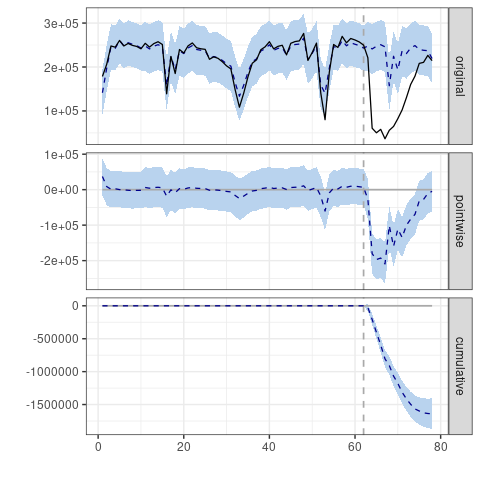
\includegraphics[width=9cm]{global_covid.png}\caption{Estimated impact of COVID pandemic.}
    \end{figure}\label{global_covid}
    \end{center}

The results in the table above show a significant reduction estimated at 44\% in the overall weekly number of medical acts in the confinement period, and a significant increase in the post-pandemic period, both in the definition of scenario 1 and scenario 2 (which excludes from the post-covid period the period of home confinement between 2020-03-14 and 2020-06-21), estimated at 18\% and 10\%, respectively.

\begin{center}
\begin{figure}[H]
  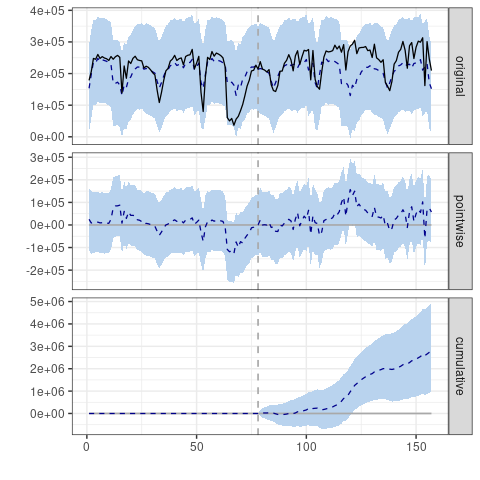
\includegraphics[width=9cm]{global_post_scen1.png}\caption{Estimated impact of post-COVID under scenario 1.}
\end{figure}\label{global_postcovid1}
\end{center}

\begin{center}
    \begin{figure}[H]
      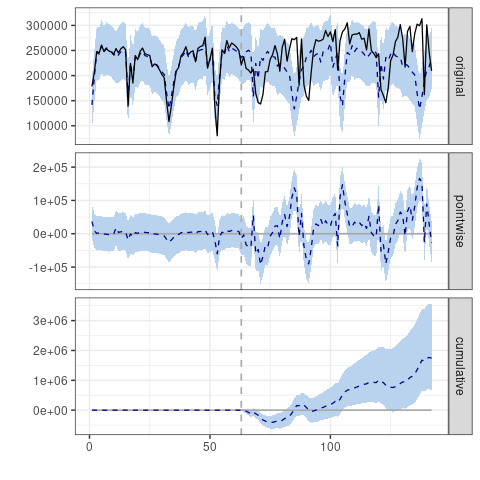
\includegraphics[width=9cm]{global_post_scen2.png}\caption{Estimated impact of post-COVID under scenario 2.}
    \end{figure}\label{global_postcovid2}
    \end{center}

The significant increase in the post-covid period in either of the two scenarios considered can be seen in Figures~\ref{global_postcovid1} and~\ref{global_postcovid2}.

\subsubsection{Global number of medical claims in Madrid}\label{md}
\begin{table}[H]\caption{Estimated impact of COVID pandemic and post-pandemic over the weekly number of medical claims in Madrid.}
  \centering  
    \begin{tabular}{ |c|c|c|c| }
        \hline
     \textbf{Scenario} & \textbf{Period} & \textbf{Relative effect (s.d.)} & \textbf{Prob. of causal effect} \\ 
     \hline
     1 & Covid-19 & -48\% (1.7\%) & 99.99\% \\  
     1 & Post-covid & 9.2\% (11\%) & 92\% \\
     \hline   
     2 & Post-covid & 1.9\% (4.6\%) & 70\% \\
     \hline
    \end{tabular}
\end{table}

\begin{center}
    \begin{figure}[H]
      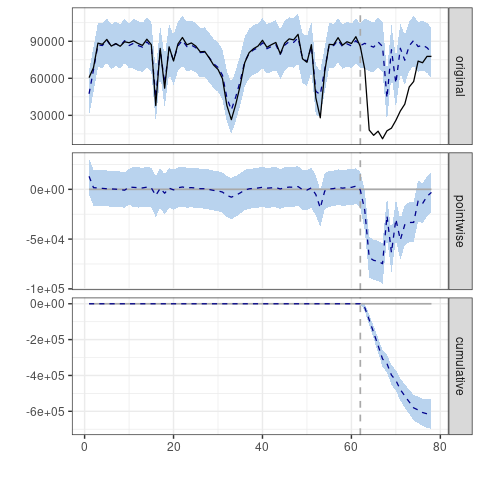
\includegraphics[width=9cm]{global_covid_Madrid.png}\caption{Estimated impact of COVID pandemic in Madrid.}
    \end{figure}
    \end{center}
    
\begin{center}
\begin{figure}[H]
  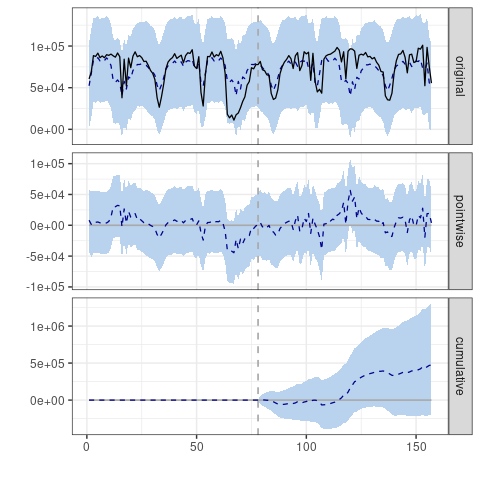
\includegraphics[width=9cm]{global_post_scen1_Madrid.png}\caption{Estimated impact of post-COVID under scenario 1 in Madrid.}
\end{figure}
\end{center}

\begin{center}
    \begin{figure}[H]
      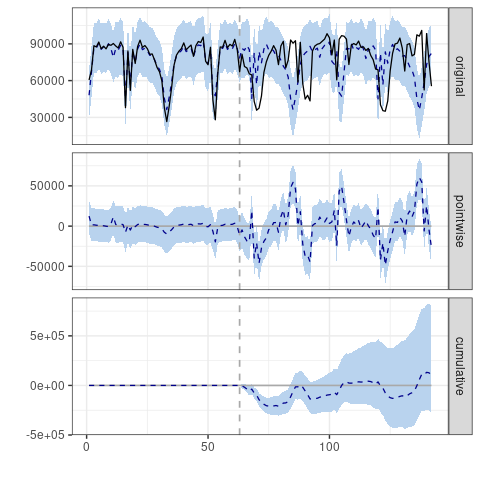
\includegraphics[width=9cm]{global_post_scen2_Madrid.png}\caption{Estimated impact of post-COVID under scenario 2 in Madrid.}
    \end{figure}
    \end{center}
    
The results show that in Madrid, in line with what was described in the previous section, there is a significant decrease in the weekly number of medical acts in the period of home confinement (estimated at around 48\%), but contrary to what was previously described, the subsequent increase (estimated at 9.2\% and 1.9\% for scenarios 1 and 2, respectively) is not significantly attributable to the consequences of the pandemic.

\subsubsection{Global number of medical claims in Barcelona}\label{bcn}
\begin{table}[H]\caption{Estimated impact of COVID pandemic and post-pandemic over the weekly number of medical claims in Barcelona.}
  \centering  
  \begin{tabular}{ |c|c|c|c| }
      \hline
   \textbf{Scenario} & \textbf{Period} & \textbf{Relative effect (s.d.)} & \textbf{Prob. of causal effect} \\ 
   \hline
   1 & Covid-19 & -46\% (2.2\%) & 99.99\% \\  
   1 & Post-covid & 26\% (13\%) &  99.66\% \\
   \hline   
   2 & Post-covid & 16\% (4.8\%) & 99.77\% \\
   \hline
  \end{tabular}
\end{table}

\begin{center}
  \begin{figure}[H]
    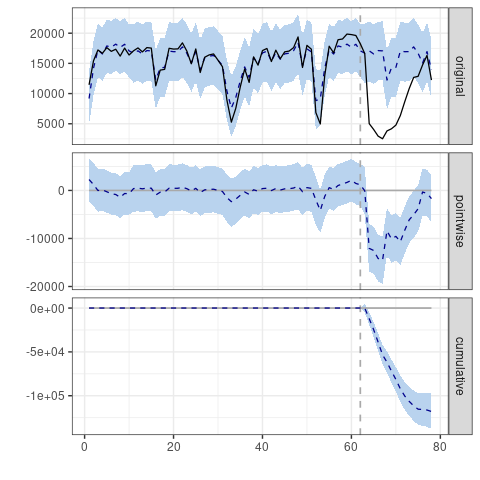
\includegraphics[width=9cm]{global_covid_Barcelona.png}\caption{Estimated impact of COVID pandemic in Barcelona.}
  \end{figure}
  \end{center}
  
\begin{center}
\begin{figure}[H]
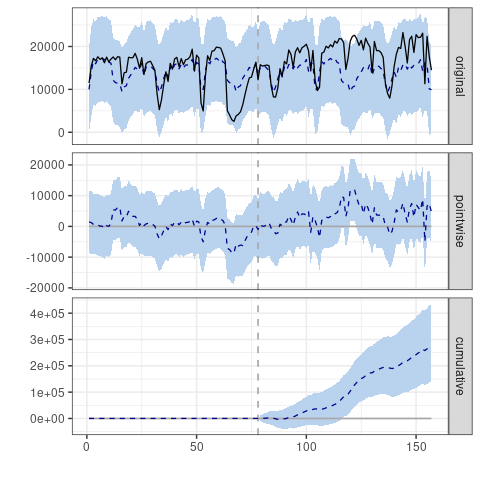
\includegraphics[width=9cm]{global_post_scen1_Barcelona.png}\caption{Estimated impact of post-COVID under scenario 1 in Barcelona.}
\end{figure}
\end{center}

\begin{center}
  \begin{figure}[H]
    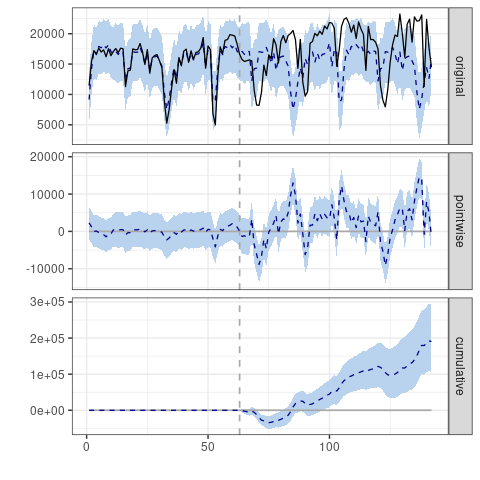
\includegraphics[width=9cm]{global_post_scen2_Barcelona.png}\caption{Estimated impact of post-COVID under scenario 2 in Barcelona.}
  \end{figure}
  \end{center}

The results show that in the province of Barcelona, in line with what occurs globally, there is a significant decrease in the weekly number of medical acts in the period of home confinement (estimated at around 46\%), and the subsequent increase (estimated at 26\% and 16\% for scenarios 1 and 2 respectively) is also significantly attributable to the consequences of the pandemic.

\subsubsection{Global number of medical claims in Valencia}\label{valencia}
\begin{table}[H]\caption{Estimated impact of COVID pandemic and post-pandemic over the weekly number of medical claims in Valencia.}
  \centering  
  \begin{tabular}{ |c|c|c|c| }
      \hline
   \textbf{Scenario} & \textbf{Period} & \textbf{Relative effect (s.d.)} & \textbf{Prob. of causal effect} \\ 
   \hline
   1 & Covid-19 & -41\% (2.1\%) & 99.99\% \\  
   1 & Post-covid & 28\% (10\%) &  99.83\% \\
   \hline   
   2 & Post-covid & 21\% (4.8\%) & 99.99\% \\
   \hline
  \end{tabular}
\end{table}

\begin{center}
  \begin{figure}[H]
    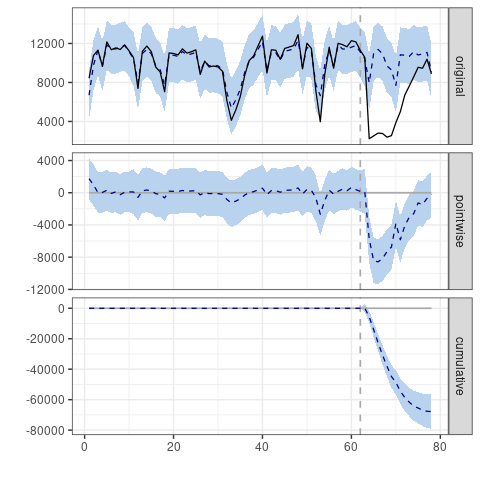
\includegraphics[width=9cm]{global_covid_Valencia.png}\caption{Estimated impact of COVID pandemic in Valencia.}
  \end{figure}
  \end{center}
  
\begin{center}
\begin{figure}[H]
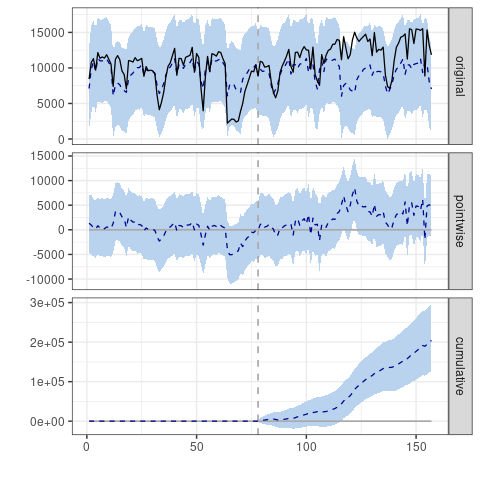
\includegraphics[width=9cm]{global_post_scen1_Valencia.png}\caption{Estimated impact of post-COVID under scenario 1 in Valencia.}
\end{figure}
\end{center}

\begin{center}
  \begin{figure}[H]
    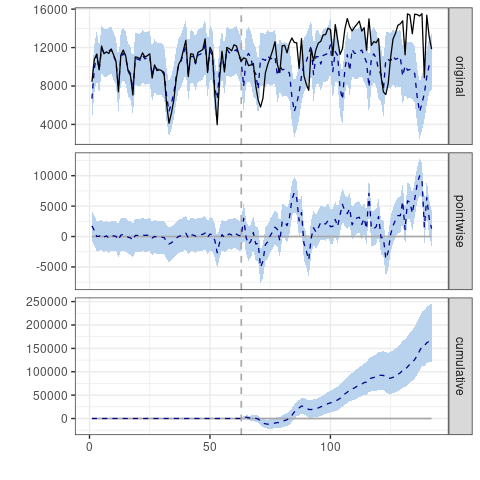
\includegraphics[width=9cm]{global_post_scen2_Valencia.png}\caption{Estimated impact of post-COVID under scenario 2 in Valencia.}
  \end{figure}
  \end{center}

The results show that in the province of Valencia, in line with what occurs globally, there is a significant decrease in the weekly number of medical acts in the period of home confinement (estimated at around 41\%), and the subsequent increase (estimated at 28\% and 21\% for scenarios 1 and 2 respectively) is also significantly attributable to the consequences of the pandemic.

\subsection{Obstetrics visits}\label{obst}
\begin{table}[H]\caption{Estimated impact of COVID pandemic and post-pandemic over the weekly number of obstetrics visits.}
  \centering  
  \begin{tabular}{ |c|c|c|c| }
      \hline
   \textbf{Scenario} & \textbf{Period} & \textbf{Relative effect (s.d.)} & \textbf{Prob. of causal effect} \\ 
   \hline
   1 & Covid-19 & -46\% (1.7\%) & 99.99\% \\  
   1 & Post-covid & 17\% (9.5\%) & 98.54\% \\
   \hline   
   2 & Post-covid & 9\% (4.3\%) & 98.52\% \\
   \hline
  \end{tabular}
\end{table}

\begin{center}
  \begin{figure}[H]
    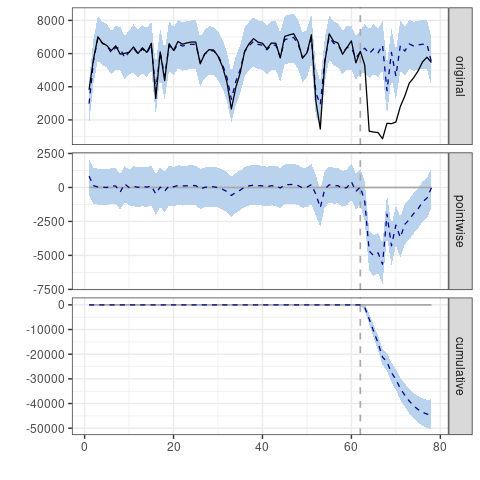
\includegraphics[width=9cm]{obstetrics_covid.png}\caption{Estimated impact of COVID pandemic over the weekly number of obstetrics visits.}
  \end{figure}
  \end{center}
  
\begin{center}
\begin{figure}[H]
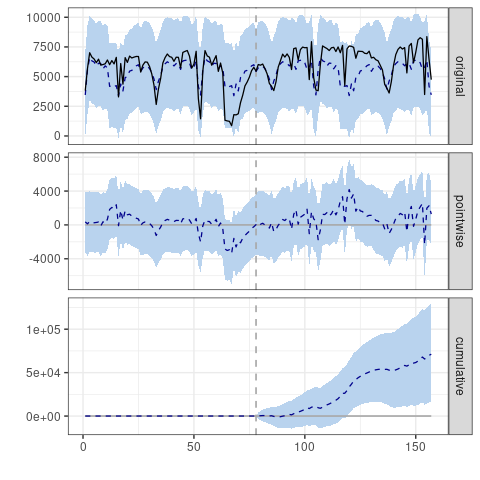
\includegraphics[width=9cm]{obstetrics_post_scen1.png}\caption{Estimated impact of post-COVID under scenario 1 over the weekly number of obstetrics visits.}
\end{figure}
\end{center}

\begin{center}
  \begin{figure}[H]
    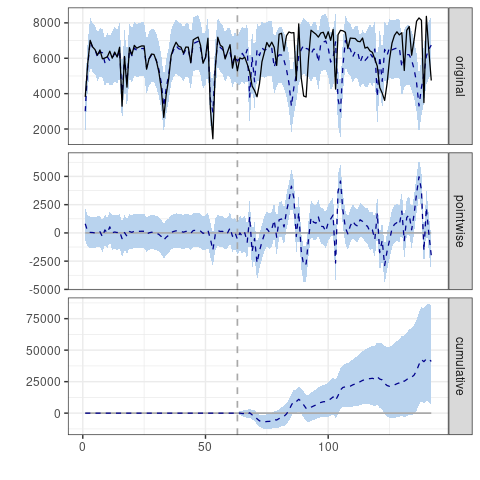
\includegraphics[width=9cm]{obstetrics_post_scen2.png}\caption{Estimated impact of post-COVID under scenario 2 over the weekly number of obstetrics visits.}
  \end{figure}
  \end{center}

Similar to what was described above, if we analyze exclusively the time series of the weekly number of visits to the obstetrics service, we also observe a significant decrease of about 46\% in the period of home confinement, and a significant increase of about 17\% or 9\% in the post-covid period, according to scenarios 1 and 2, respectively. 

\subsubsection{Obstetrics visits in Madrid}\label{md}
\begin{table}[H]\caption{Estimated impact of COVID pandemic and post-pandemic over the weekly number of obstetrics visits in Madrid.}
  \centering
    \begin{tabular}{ |c|c|c|c| }
      \hline
   \textbf{Scenario} & \textbf{Period} & \textbf{Relative effect (s.d.)} & \textbf{Prob. of causal effect} \\ 
   \hline
   1 & Covid-19 & -51\% (1.4\%) & 99.99\% \\  
   1 & Post-covid & 11\% (9.9\%) & 94\% \\
   \hline   
   2 & Post-covid & 2.6\% (4.3\%) & 79\% \\
   \hline
  \end{tabular}
\end{table}

\begin{center}
  \begin{figure}[H]
    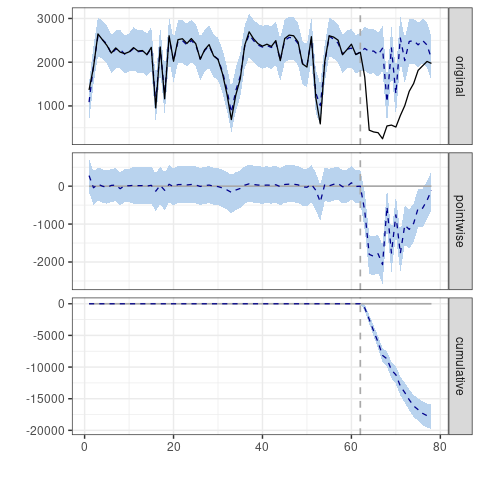
\includegraphics[width=9cm]{obstetrics_covid_Madrid.png}\caption{Estimated impact of COVID pandemic over the weekly number of obstetrics visits in Madrid.}
  \end{figure}
  \end{center}
  
\begin{center}
\begin{figure}[H]
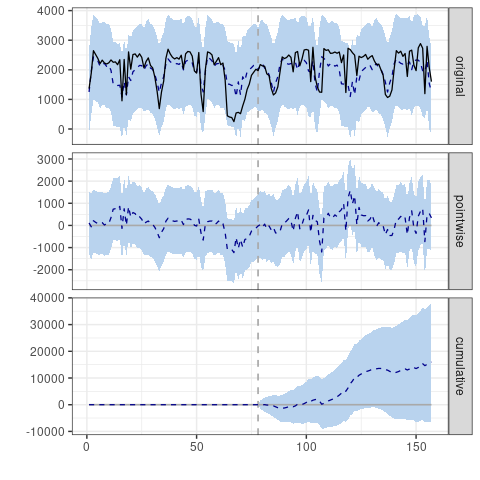
\includegraphics[width=9cm]{obstetrics_post_scen1_Madrid.png}\caption{Estimated impact of post-COVID under scenario 1 over the weekly number of obstetrics visits in Madrid.}
\end{figure}
\end{center}

\begin{center}
  \begin{figure}[H]
    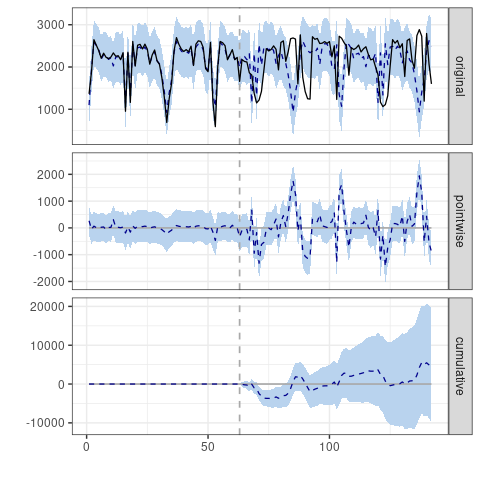
\includegraphics[width=9cm]{obstetrics_post_scen2_Madrid.png}\caption{Estimated impact of post-COVID under scenario 2 over the weekly number of obstetrics visits in Madrid.}
  \end{figure}
  \end{center}

With respect to the analysis of the evolution of the weekly number of visits to the obstetrics service in the province of Madrid, the results show that in Madrid, in line with what was described in the previous section, there was a significant decrease in the weekly number of medical acts in the period of home confinement (estimated at around 48\%), but contrary to what was previously described, the subsequent increase (estimated at 9.2\% and 1.9\% for scenarios 1 and 2 respectively) is not significantly attributable to the consequences of the pandemic.

\subsubsection{Obstetrics visits in Barcelona}\label{bcn}
\begin{table}[H]\caption{Estimated impact of COVID pandemic and post-pandemic over the weekly number of obstetrics visits in Barcelona.}
  \centering  
  \begin{tabular}{ |c|c|c|c| }
      \hline
   \textbf{Scenario} & \textbf{Period} & \textbf{Relative effect (s.d.)} & \textbf{Prob. of causal effect} \\ 
   \hline
   1 & Covid-19 & -43\% (2.3\%) & 99.99\% \\  
   1 & Post-covid & 24\% (9.2\%) & 99.53\% \\
   \hline   
   2 & Post-covid & 17\% (5\%) & 99.53\% \\
   \hline
  \end{tabular}
\end{table}

\begin{center}
  \begin{figure}[H]
    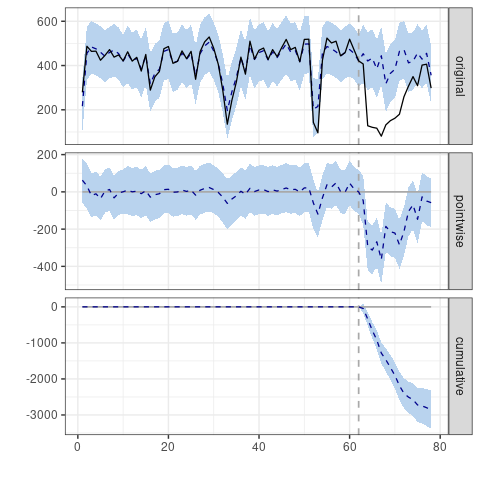
\includegraphics[width=9cm]{obstetrics_covid_Barcelona.png}\caption{Estimated impact of COVID pandemic over the weekly number of obstetrics visits in Barcelona.}
  \end{figure}
  \end{center}
  
\begin{center}
\begin{figure}[H]
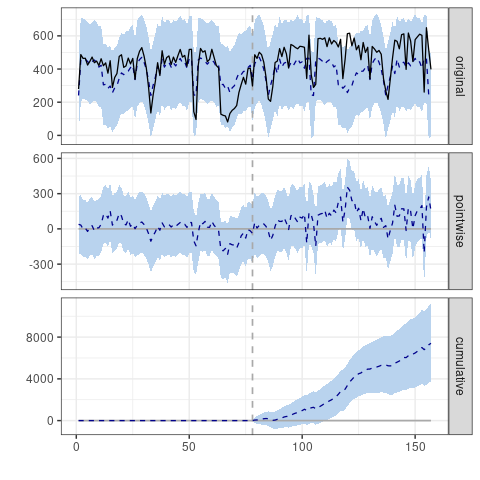
\includegraphics[width=9cm]{obstetrics_post_scen1_Barcelona.png}\caption{Estimated impact of post-COVID under scenario 1 over the weekly number of obstetrics visits in Barcelona.}
\end{figure}
\end{center}

\begin{center}
  \begin{figure}[H]
    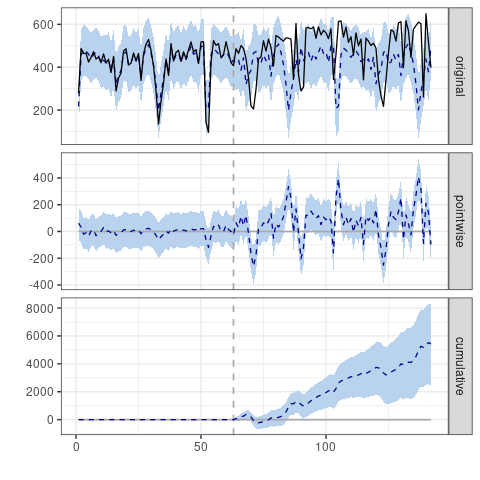
\includegraphics[width=9cm]{obstetrics_post_scen2_Barcelona.png}\caption{Estimated impact of post-COVID under scenario 2 over the weekly number of obstetrics visits in Barcelona.}
  \end{figure}
  \end{center}

Regarding the analysis of the evolution of the weekly number of visits to the obstetrics service in the province of Barcelona, the results show that, in line with what has been described above, there was a significant decrease in the weekly number of medical acts in the period of home confinement (estimated at around 43\%) and the subsequent increase (estimated at 24\% and 17\% for scenarios 1 and 2, respectively) is also significantly attributable to the consequences of the pandemic.

\subsubsection{Obstetrics visits in Valencia}\label{valencia}
\begin{table}[H]\caption{Estimated impact of COVID pandemic and post-pandemic over the weekly number of obstetrics visits in Valencia.}
\centering
  \begin{tabular}{ |c|c|c|c| }
      \hline
   \textbf{Scenario} & \textbf{Period} & \textbf{Relative effect (s.d.)} & \textbf{Prob. of causal effect} \\ 
   \hline
   1 & Covid-19 & -42\% (2.5\%) & 99.99\% \\  
   1 & Post-covid & 32\% (9.1\%) & 99.78\% \\
   \hline   
   2 & Post-covid & 24\% (5\%) & 99.89\% \\
   \hline
  \end{tabular}
\end{table}

\begin{center}
  \begin{figure}[H]
    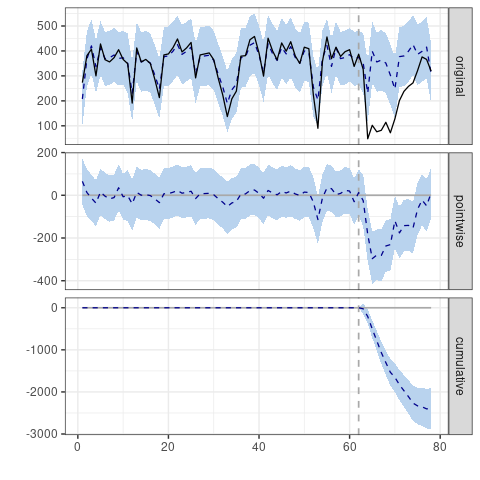
\includegraphics[width=9cm]{obstetrics_covid_Valencia.png}\caption{Estimated impact of COVID pandemic over the weekly number of obstetrics visits in Valencia.}
  \end{figure}
  \end{center}
  
\begin{center}
\begin{figure}[H]
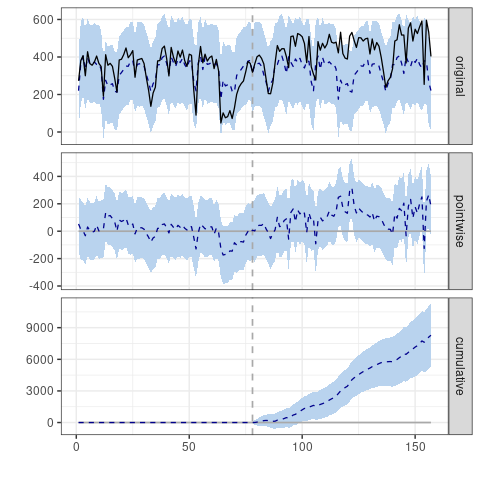
\includegraphics[width=9cm]{obstetrics_post_scen1_Valencia.png}\caption{Estimated impact of post-COVID under scenario 1 over the weekly number of obstetrics visits in Valencia.}
\end{figure}
\end{center}

\begin{center}
  \begin{figure}[H]
    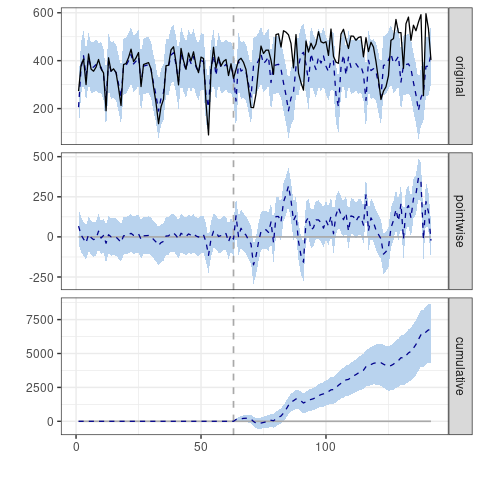
\includegraphics[width=9cm]{obstetrics_post_scen2_Valencia.png}\caption{Estimated impact of post-COVID under scenario 2 over the weekly number of obstetrics visits in Valencia.}
  \end{figure}
  \end{center}

  Regarding the analysis of the evolution of the weekly number of visits to the obstetrics service in the province of Valencia, the results show that, in line with what has been described above, there was a significant decrease in the weekly number of medical acts in the period of home confinement (estimated at around 42\%) and the subsequent increase (estimated at 32\% and 24\% for scenarios 1 and 2, respectively) is also significantly attributable to the consequences of the pandemic.

%\bibliography{sample}
\end{document}
